\documentclass[a4paper,12pt]{article}
\usepackage[utf8]{inputenc}
\usepackage{listings}
\usepackage{float}
\usepackage[margin=1in]{geometry}
\setlength\parindent{0pt}
\usepackage{xcolor}
\usepackage{graphicx}
\definecolor{dkgreen}{rgb}{0,0.6,0}
\definecolor{dred}{rgb}{0.545,0,0}
\definecolor{dblue}{rgb}{0,0,0.545}
\definecolor{lgrey}{rgb}{0.9,0.9,0.9}
\definecolor{gray}{rgb}{0.4,0.4,0.4}
\definecolor{darkblue}{rgb}{0.0,0.0,0.6}
\lstdefinelanguage{python}{
      backgroundcolor=\color{lgrey},  
      basicstyle=\footnotesize \ttfamily \color{black} \bfseries,   
      breakatwhitespace=false,       
      breaklines=true,               
      captionpos=b,                   
      commentstyle=\color{dkgreen},   
      deletekeywords={...},          
      escapeinside={\%*}{*)},                  
      frame=single,                  
      language=C++,                
      keywordstyle=\color{purple},  
      morekeywords={BRIEFDescriptorConfig,string,TiXmlNode,DetectorDescriptorConfigContainer,istringstream,cerr,exit}, 
      identifierstyle=\color{black},
      stringstyle=\color{blue},      
      numbers=right,                 
      numbersep=5pt,                  
      numberstyle=\tiny\color{black}, 
      rulecolor=\color{black},        
      showspaces=false,               
      showstringspaces=false,        
      showtabs=false,                
      stepnumber=1,                   
      tabsize=5,                     
      title=\lstname,                 
    }
    
%opening
\title{CS325 Homework 1}
\author{Kabir Kang, Paul Ely, Jason Dorweiler}

\begin{document}

\maketitle

\section*{Mathematical Analysis}
  \begin{lstlisting}[language=python,caption={pseudo code for $n^3$ algorithm}]
if len(array) == 1:
	maxSum = array[0]
else:
	for e in range(len(array)):
		for j in range(e,len(array)):
			maxSum = np.maximum(maxSum, sum(array[e:j]))
  \end{lstlisting}
  
  \begin{lstlisting}[language=python,caption={pseudo code for $n^2$ algorithm}]
for e in range(len(array)):
	testSum = 0
	for j in range(e,len(array)):
		testSum += array[j]
		maxSum = np.maximum(maxSum, testSum)
  \end{lstlisting}

  \begin{lstlisting}[language=python,caption={pseudo code for $n\log(n)$ algorithm}]
def algo3(array):
if(len(array) == 0):
	return 0
if(len(array) == 1):
	return array[0]

mid = len(array)/2
tempL = tempR = 0
maxLeft = maxRight = -99999

#left side crossing -- mid backwards
for i in range(mid,0,-1):
	tempL = tempL + array[i]
	maxLeft = np.maximum(maxLeft, tempL)

#right side crossing -- mid forwards
for j in range(mid+1, len(array)):
	tempR = tempR + array[j]
	maxRight = np.maximum(maxRight, tempR)
maxCrossing = maxLeft + maxRight

MaxA = algo3(array[:mid])
MaxB = algo3(array[mid+1:])

return np.maximum(np.maximum(MaxA, MaxB),maxCrossing))
  \end{lstlisting} 

\section*{Theoretical Correctness}

\section*{Experimental Analysis}

\begin{figure}[h!]
\centering
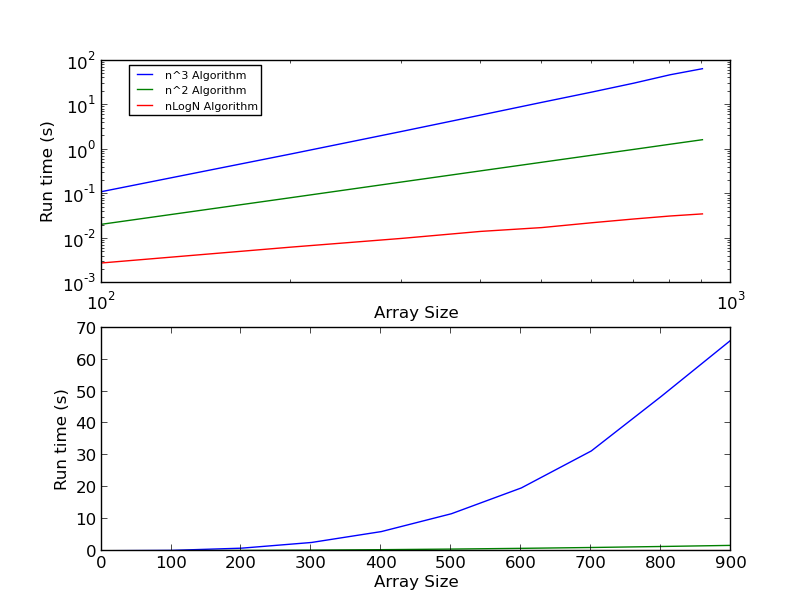
\includegraphics[width=0.8\textwidth]{plotTo900}
\caption{Plot of the three algorithms up to array size of 900, top: log/log, bottom: normal axis}
\end{figure} 

A plot of the run times for the three algorithms are shown in figure 1.  The results of the slope calculation for each algorithm are shown in the table below.  The slope calculation fits with what we would expect.  The $n^3$ algorithm has a slope ~3, the $n^2$ algorithem has a slope ~2, and the $n\log(n)$ algorithm has a slope a bit higher than 1. \\

\begin{tabular}{|c|c|}
\hline 
Algorithm & Slope of log-log plot \\ 
\hline 
$n^3$ & 2.89 \\ 
\hline 
$n^2$ & 1.99 \\ 
\hline 
$n\log(n)$ & 1.16 \\ 
\hline 
\end{tabular}\\

In the lower plot on figure 1 we have also plotted the three algorithms with a normal axis.  This shows the $n^3$ run time of the first algorithm.  The third algorithm runs so quickly that it doesn't even show up at this scale. 

\begin{figure}[h!]
\centering
\includegraphics[width=0.8\textwidth]{plotTo9000}
\caption{Plot of the three algorithms up to array size of 9000, top: log/log, bottom: normal axis}
\end{figure} 



\pagebreak
 

\section*{Extrapolation and Interpretation}

\textbf{What is the biggest instance that you could solve with your algorithm in one hour}\\


\textbf{Determine the slope of the line in your log-log plot and from these slopes infer the experimental running time for each algorithm. Discuss any discrepancies between the experimental and theoretical running times}\\

\end{document}
